%!TEX encoding = UTF-8 Unicode
\documentclass{article}[encoding=U]
\usepackage{listings}
\usepackage{xcolor}
\usepackage{titling}
\usepackage{graphicx}
\usepackage[bottom]{footmisc}
\usepackage{hyperref}


\newcommand{\logo}[1]{%
	\postauthor{%
	\end{tabular}\par\end{center}
\begin{center}\includegraphics[scale=0.8]{#1}\end{center}
\vskip0.5em}%
}

%%%%%%%%%%%%%%%%%%%%%%%%%%%%%%%%%%%%
%   CONFIGURAZIONI
%%%%%%%%%%%%%%%%%%%%%%%%%%%%%%%%%%%%
\title{
	TURING \\
	\large disTribUted collaboRative edItiNG \\
	\large Reti di Calcolatori - Laboratorio}
\author{
	Federico Gerardi \\
	Matricola: 508082 \\
	\texttt{federicogerardi94@gmail.com}}
\logo{assets/logo}

\lstset{
	basicstyle=\footnotesize,
	aboveskip=0.5cm,
	belowskip=0.5cm,
	showstringspaces=false,
	keywordstyle=\bfseries,
	numbers=none,
	breaklines=true,
	rangeprefix = \#,
	includerangemarker = false
}
\lstdefinelanguage{JSON}{%
	keywords={true, false, null, undefined},
	keywordstyle=\bfseries,
	ndkeywordstyle=\bfseries,
	sensitive=false,
	comment=[l]{//},
	morecomment=[s]{/*}{*/},
	commentstyle=\ttfamily,
	stringstyle=\color{blue}\ttfamily,
	morestring=[b]',
	morestring=[b]`,
	morestring=[b]"
}
\definecolor{lightgray}{gray}{0.95}

\begin{document}
\maketitle
\bigskip
\begin{abstract}
TURING - \textit{disTribUted collaboRative edItiNG} è una piattaforma client-server realizzata come progetto finale per il modulo di Laboratorio dell'esame di Reti di Calcolatori della Laurea Triennale in informatica dell'Università di Pisa. Il progetto si basa sulla creazione di un sistema di document editing multiutente distribuito (simile a quello offerto da Docs di Google), che gestisce permessi di modifica e operazioni di aggiornamento dei contenuti dei documenti esistenti in maniera concorrente e consistente. Questo paper fornirà una panoramica della sua infrastruttura e illustrerà alcune scelte implementative.
\end{abstract}

\newpage

\tableofcontents
\clearpage

\section{Funzioni della piattaforma}
Le funzionalità che la piattaforma implementa sono le seguenti:
\begin{itemize}
	\item Creazione di un nuovo utente;
	\item Login dell'utente all'interno della piattaforma;
	\item Inizio della fase di modifica di una specifica sezione di un documento;
	\item Terminazione della fase di modifica e aggiornamento della relativa sezione sul server;
	\item Visualizzazione di una sezione del documento;
	\item Visualizzazione di un intero documento
	\item Operazioni per l'invio/ricezione di messaggi in chat condivisa tra gli editor di più sezioni appartenenti allo stesso documento.
	\item Condivisione dei permessi di accesso ad un documento di cui si è i proprietari ad altri utenti;
	\item Gestione delle notifiche generate in seguito alla ricezione dei permessi di accesso ad un documento.
\end{itemize}

\section{Esecuzione dell'Applicazione}
\subsection{Compilazione}
La compilazione viene gestita attraverso il toolkit \textit{Maven}, che ci permette di definire delle apposite routine\footnote{È definita anche una routine per \textit{pulire}} che si occuperanno di effettuare il packing sia del client che del server di TURING.\\


\subsection{Server}
\subsection{Client}

\section{Interfaccia utente}
\subsection{Argomenti a Linea di Comando}
Utilizzando alcuni argomenti da linea di comando, è possibile specificare alcune preferenze\footnote{È possibile avere la lista completa attraverso l'invocazione dei due programmi con il flag \textit{-h} o \textit{--help} } del comportamento sia del client che del server. \\
In particolare, le seguenti sono i parametri di connessione personalizzabili attraverso gli argomenti a riga di comando:

\begin{itemize}
	\item\textit{--tcp-command-port}: Numero di porta utilizzato per la connessione relativa allo scambio di comando/responso;
	\item\textit{--udp-multicast-port}: Numero di porta utilizzato\footnote{Opzione disponibile unicamente sul client} per lo scambio di messaggi multicast;
	\item\textit{--rmi-port}: Numero di porta utilizzato per la connessione TCP sfruttata per effettuare chiamate RMI\footnote{L'unica funzione che sfrutta RMI è la registrazione di nuovi utenti};
	\item\textit{-data-dir}: Path utilizzato per effettuare la memorizzazione dei dati\footnote{Viene utilizzato dal client per memorizzare i file locali delle sezioni in modifica e dal server per memorizzare la serializzazione degli oggetti utili al mantenimento dei dati relativi agli utenti e ai documenti};
	\item\textit{--server-address}: Indirizzo IPv4 del server\footnote{Opzione disponibile unicamente sul client};
	\item\textit{--config-file}: Nome del file JSON di configurazione;
\end{itemize}
\paragraph{File JSON di Configurazione}
Per non dover utilizzare molti argomenti da riga di comando in ambienti in cui sorge la necessità di utilizzare molti parametri i cui valori differiscono da quelli di default, TURING mette a disposizione\footnote{Sia il client, che il server mettono a disposizione questa funzionalità} la possibilità di utilizzare un file JSON di configurazione da passare come unico argomento a riga di comando durante l'esecuzione dell'applicazione.
\newline
Le stringhe utilizzabili all'interno dell'oggetto JSON principale sono le seguenti\footnote{Corrispondono a quelle illustrate precedentemente come argomenti a linea di comando}:
\begin{itemize}
	\item \textit{TCP\_PORT}
	\item \textit{UDP\_PORT}
	\item \textit{RMI\_PORT}
	\item \textit{DATA\_DIR}
	\item \textit{SERVER\_ADDRESS}
\end{itemize}

\begin{lstlisting}[caption="JSON File - Esempio", language=JSON]
{
	"TCP_PORT": 9658,
	"DATA_DIR": "/home/user/TURING/",
	"RMI_PORT": 15698
}
\end{lstlisting}

\subsection{CLI}
È possibile interagire con il sistema attraverso l'apposito client. Questo fornisce un interfaccia interattiva a riga di comando, con la quale è possibile interagire grazie all'inserimento iterativo di comandi utilizzando il relativo prompt.

\begin{figure}[h]
	\caption{TURING Client - Esempio del prompt}
	\centering
		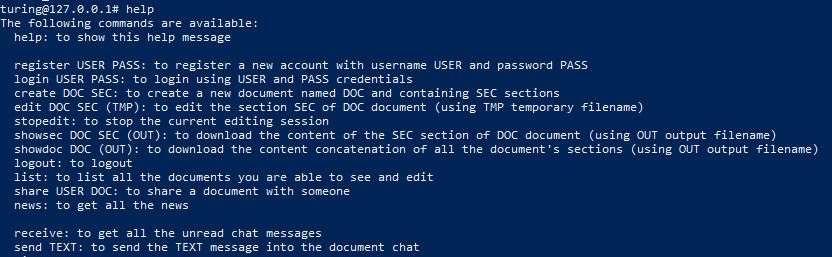
\includegraphics[width=0.8\linewidth]{assets/help_message}
\end{figure}


\section{Struttura dei Package}
I package principali, figli del root package \textit{it.azraelsec}, che fanno parte del progetto sono i seguenti:
\begin{itemize}
	\item \texttt{Chat} - Cassi che interessate nella gestione del servizio di messaggistica multicast UDP
	\item \texttt{Client} - Classi costituenti il client del sistema TURING
	\item \texttt{Document} - Classi relativi alla rappresentazione dei documenti e delle sezioni costituenti\footnote{I Documenti, infatti, sono formati in realtà da un'aggreazione di differenti Sezioni}
	\item \texttt{Notification} - Classi per la gestione delle notifiche lato client e per la loro generazione lato server
	\item \texttt{Protocol} - Classi ed interfacce atte alla gestione del protocollo di rete \textit{low-level}
	\item \texttt{Server} - Classi costituenti il server del sistema TURING, relative alla gestione del concetto di \textit{Utente} ed al ciclo di vita delle sue sessioni
\end{itemize}
\begin{figure}[h]
	\caption{UML - Package Diagram}
	\centering
	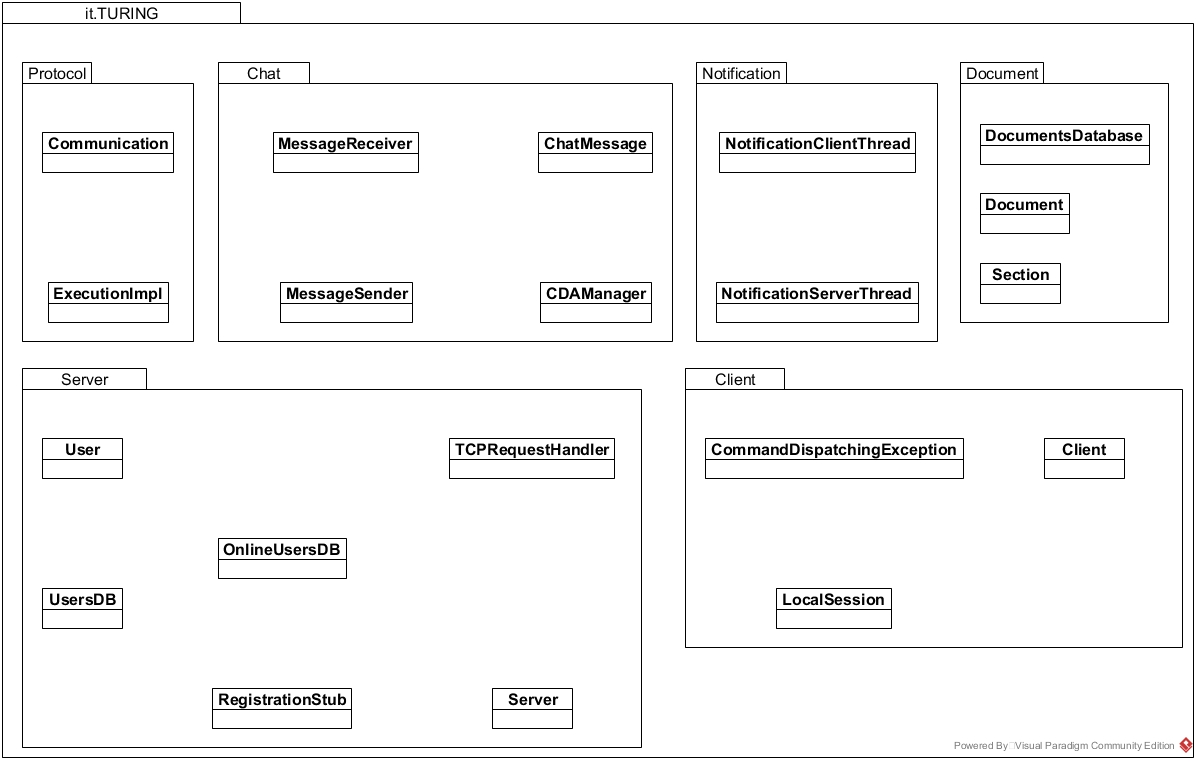
\includegraphics[width=1\linewidth]{assets/package_diagram}
\end{figure}

\pagebreak


\section{Server}


\end{document}

